% Olympus v2 — simplified system architecture (thin banner variant)
% arch_thin.tex — same content as architecture_simplified.tex but laid out
% as a single horizontal band (env | agent | learner | orchestrator) so the
% figure is much wider and shorter: the control plane no longer sits on a
% second row; the "start episodes" edge is routed along a rail over the top.
% Compile standalone:  pdflatex arch_thin.tex
\documentclass[tikz,border=5pt]{standalone}
\usepackage{tikz}
\usepackage{amssymb}
\usepackage{helvet}
\renewcommand{\familydefault}{\sfdefault}
\usetikzlibrary{arrows.meta,positioning,fit,backgrounds}

\begin{document}
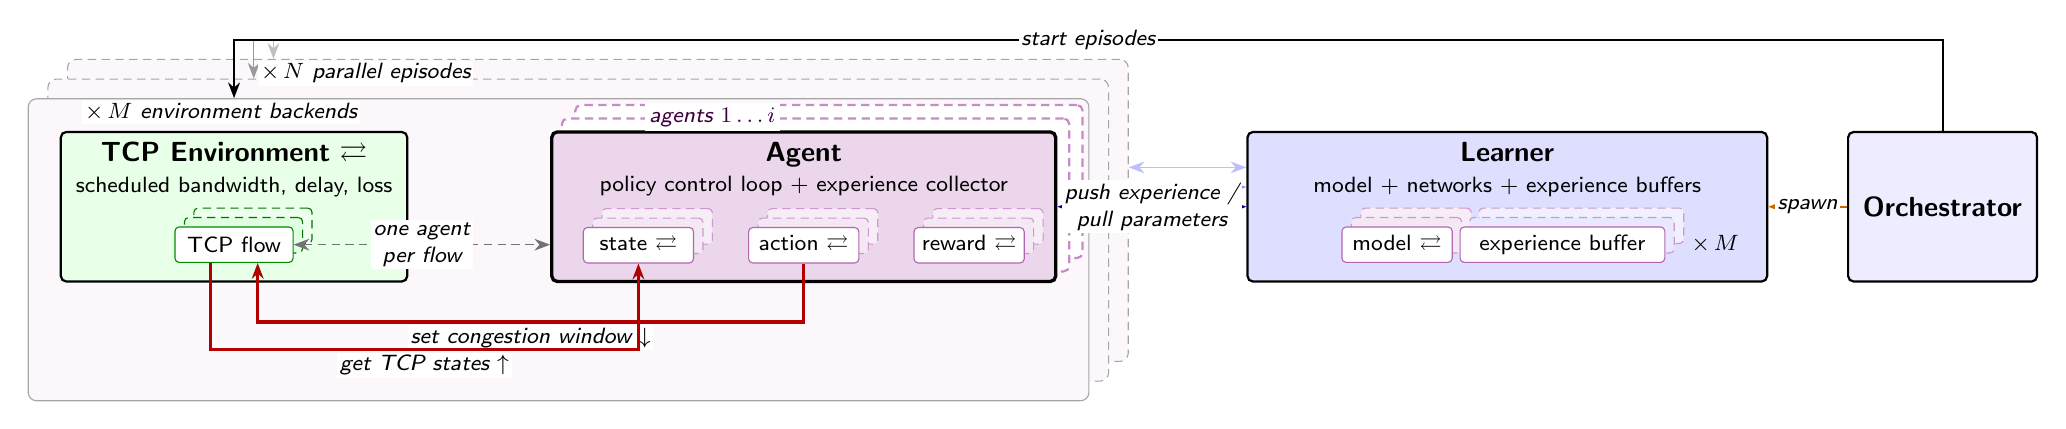
\begin{tikzpicture}[
  font=\normalsize,
  node distance=11mm and 22mm,
  >={Stealth[length=2mm]},
  proc/.style={draw,rounded corners=2pt,thick,minimum height=8mm,
               minimum width=24mm,align=center,fill=blue!7},
  net/.style={draw,rounded corners=2pt,thick,minimum height=8mm,
              minimum width=30mm,align=center,fill=green!9},
  agent/.style={proc,fill=violet!16,very thick},
  card/.style={draw,rounded corners=3pt,thin,draw=black!35,fill=violet!3},
  ghostcard/.style={draw,densely dashed,rounded corners=3pt,thin,
                    draw=black!35,fill=violet!3},
  subbox/.style={draw,rounded corners=1.5pt,thin,draw=violet!60,fill=white,
                 font=\footnotesize,inner sep=2pt,
                 minimum width=14mm,minimum height=4.5mm},
  subbg/.style={draw,densely dashed,rounded corners=1.5pt,thin,
                draw=violet!40,fill=white,
                font=\footnotesize,inner sep=2pt,
                minimum width=14mm,minimum height=4.5mm},
  flowbox/.style={draw,rounded corners=1.5pt,thin,draw=green!55!black,fill=white,
                 font=\footnotesize,inner sep=2pt,
                 minimum width=15mm,minimum height=4.5mm},
  flowbg/.style={draw,densely dashed,rounded corners=1.5pt,thin,
                draw=green!45!black,fill=white,
                font=\footnotesize,inner sep=2pt,
                minimum width=15mm,minimum height=4.5mm},
  maonly/.style={draw=violet!45,densely dashed,thick,rounded corners=2pt,
                 fill=violet!7},
  ctrl/.style={->,thick},
  data/.style={->,very thick,draw=red!70!black},
  tap/.style={->,thin,draw=red!55!black},
  ipc/.style={<->,thick,draw=blue!60!black},
  cfg/.style={->,thick,draw=orange!80!black},
  lbl/.style={font=\footnotesize\itshape,fill=white,inner sep=1pt},
]

% ---- single band, left to right: env | agent | learner | orchestrator ----
\node[net,minimum width=44mm,minimum height=19mm] (env) {};
\node[align=center,anchor=north,inner sep=0pt] at ([yshift=-1.4mm]env.north)
     {\textbf{TCP Environment} $\rightleftarrows$\\[-1pt]\footnotesize scheduled bandwidth, delay, loss};

% dashed background copies of the env -- one per environment (x M)
\begin{scope}[on background layer]
  \node[draw,densely dashed,thin,rounded corners=2pt,draw=green!50!black,
        fill=green!6,minimum width=44mm,minimum height=19mm]
        at ([xshift=2.4mm,yshift=2.4mm]env) {};
  \node[draw,densely dashed,thin,rounded corners=2pt,draw=green!50!black,
        fill=green!8,minimum width=44mm,minimum height=19mm]
        at ([xshift=1.2mm,yshift=1.2mm]env) {};
\end{scope}
\node[font=\footnotesize\itshape,anchor=south west,fill=white,inner sep=1pt]
      at ([xshift=2.8mm,yshift=0.8mm]env.north west)
      {$\times\,M$ environment backends};

% tcp flow deck inside the env: stacked cards = possibly several flows
\node[flowbg,anchor=south,fill=green!7] at ([xshift=2.4mm,yshift=4.9mm]env.south) {};
\node[flowbg,anchor=south,fill=green!12] at ([xshift=1.2mm,yshift=3.7mm]env.south) {};
\node[flowbox,anchor=south] at ([xshift=0mm,yshift=2.5mm]env.south) (tcpflow) {TCP flow};

% agent shell, with internal state + action + reward module decks
\node[agent,right=18mm of env,minimum width=64mm,minimum height=19mm] (worker) {};
\node[align=center,anchor=north,inner sep=0pt] at ([yshift=-1.4mm]worker.north)
     {\textbf{Agent}\\[-1pt]\footnotesize policy control loop + experience collector};

% three swappable module decks across the agent bottom: state | action | reward

% -- state
\node[subbg,anchor=south,fill=violet!7] at ([xshift=-18.6mm,yshift=4.9mm]worker.south) {};
\node[subbg,anchor=south,fill=violet!9] at ([xshift=-19.8mm,yshift=3.7mm]worker.south) {};
\node[subbox,anchor=south] at ([xshift=-21mm,yshift=2.5mm]worker.south) (wstate) {state $\rightleftarrows$};

% -- action
\node[subbg,anchor=south,fill=violet!7] at ([xshift=2.4mm,yshift=4.9mm]worker.south) {};
\node[subbg,anchor=south,fill=violet!9] at ([xshift=1.2mm,yshift=3.7mm]worker.south) {};
\node[subbox,anchor=south] at ([xshift=0mm,yshift=2.5mm]worker.south) (waction) {action $\rightleftarrows$};

% -- reward
\node[subbg,anchor=south,fill=violet!7] at ([xshift=23.4mm,yshift=4.9mm]worker.south) {};
\node[subbg,anchor=south,fill=violet!9] at ([xshift=22.2mm,yshift=3.7mm]worker.south) {};
\node[subbox,anchor=south] at ([xshift=21mm,yshift=2.5mm]worker.south) (wreward) {reward $\rightleftarrows$};

% ---- control plane continues the same row ----
\node[proc,right=24mm of worker,fill=blue!13,minimum width=66mm,minimum height=19mm] (learner) {};
\node[align=center,anchor=north,inner sep=0pt] at ([yshift=-1.4mm]learner.north)
     {\textbf{Learner}\\[-1pt]\footnotesize model + networks + experience buffers};

% model deck (left) inside the learner
\node[subbg,anchor=south,fill=violet!7] at ([xshift=-11.6mm,yshift=4.9mm]learner.south) {};
\node[subbg,anchor=south,fill=violet!9] at ([xshift=-12.8mm,yshift=3.7mm]learner.south) {};
\node[subbox,anchor=south] at ([xshift=-14mm,yshift=2.5mm]learner.south) (lmodel) {model $\rightleftarrows$};

% experience buffers: a solid pile of identical buffers -- one per environment.
\node[subbg,anchor=south,fill=blue!6,minimum width=26mm] at ([xshift=9.4mm,yshift=4.9mm]learner.south) {};
\node[subbg,anchor=south,fill=blue!9,minimum width=26mm] at ([xshift=8.2mm,yshift=3.7mm]learner.south) {};
\node[subbox,anchor=south,minimum width=26mm] at ([xshift=7mm,yshift=2.5mm]learner.south) (lbuffer) {experience buffer};
\node[font=\footnotesize\itshape,anchor=west,inner sep=1pt] at ([xshift=23mm,yshift=4.9mm]learner.south) {$\times\,M$};

\node[proc,minimum height=19mm,right=10mm of learner] (orch) {\textbf{Orchestrator}};

% rail height for the "start episodes" edge, routed over the top of the band
\coordinate (railtop) at ([yshift=11.5mm]orch.north);

% area reserved below the decks so the control-loop arrows stay inside the card
\coordinate (dataarea) at ([yshift=-11mm]env.south);

% ---- stack the rollout row into N parallel episodes ----
\begin{scope}[on background layer]
  % rear wide boxes are dashed
  \node[ghostcard,fit=(env)(worker)(dataarea),inner sep=4mm,xshift=5mm,yshift=5mm]   (roll3) {};
  \node[ghostcard,fit=(env)(worker)(dataarea),inner sep=4mm,xshift=2.5mm,yshift=2.5mm] (roll2) {};

  % front wide box is solid
  \node[card,fit=(env)(worker)(dataarea),inner sep=4mm] (rollout) {};

  % faint fan-out onto the other stacked rollouts
  \coordinate (e1) at (rollout.north -| env);
  \coordinate (w1) at (rollout.east |- worker);

  \draw[->,thin,draw=black!40]
        ([xshift=2.5mm]e1 |- railtop) -- ([shift={(2.5mm,2.5mm)}]e1);

  \draw[->,thin,draw=black!25]
        ([xshift=5mm]e1 |- railtop) -- ([shift={(5mm,5mm)}]e1);

  \draw[<->,thin,draw=blue!42]
        ([yshift=2.5mm]learner.west) -- ([shift={(2.5mm,2.5mm)}]w1);

  \draw[<->,thin,draw=blue!26]
        ([yshift=5mm]learner.west) -- ([shift={(5mm,5mm)}]w1);
\end{scope}

% "x N parallel episodes" -- marks the stacked rollout cards.
\node[font=\footnotesize\itshape,anchor=south west,fill=white,inner sep=1pt]
      at ([xshift=3mm,yshift=1.5mm]rollout.north -| env)
      {$\times\,N$ parallel episodes};

% ---- extra agents -- present ONLY in the multi-agent case ----
\begin{scope}[on background layer]
  \node[maonly,fit=(worker),inner sep=0mm,xshift=3.2mm,yshift=3.2mm,fill=white] (maWorkerB) {};
  \node[maonly,fit=(worker),inner sep=0mm,xshift=1.5mm,yshift=1.5mm,fill=white] (maWorkerA) {};
\end{scope}

\node[font=\footnotesize\itshape,text=violet!50!black,anchor=east,fill=white,inner sep=1.5pt]
     at ([xshift=-3mm,yshift=1.7mm]worker.north) {agents $1\ldots i$};

% ===== edges =====
\draw[cfg] (orch) -- node[lbl]{spawn} (learner);

% start episodes: up from the orchestrator, along the top rail, down into
% the rollout card above the environment.
\draw[ctrl] (orch.north) -- (orch.north |- railtop)
      -- node[lbl,pos=0.5]{start episodes} (e1 |- railtop)
      -- (e1);

\draw[ipc] (worker) --
      node[lbl,align=center]{push experience /\\pull parameters}
      (learner);

% the control loop lives between the agent and the environment's tcp flow(s).
% Right-angle (orthogonal) routing: two 90-degree turns per line. The lines are
% NESTED -- the lower getsockopt line brackets the upper setsockopt line on both
% sides -- so they never cross or overlap. Both terminate on the tcp flow deck.
% Both lines (and their labels) are routed inside the rollout card.
\coordinate (setline) at ([yshift=-5mm]env.south);
\coordinate (getline) at ([yshift=-8.5mm]env.south);

% setsockopt(cwnd): agent action deck -> tcp flow   (upper line)
\draw[data,->] (waction.south) -- (waction.south |- setline)
      -- node[lbl,below=0.2mm]{set congestion window $\downarrow$}
         ([xshift=3mm]tcpflow.south |- setline)
      -- ([xshift=3mm]tcpflow.south);

% getsockopt(tcp_info): tcp flow -> agent state deck   (lower line)
\draw[data,->] ([xshift=-3mm]tcpflow.south) -- ([xshift=-3mm]tcpflow.south |- getline)
      -- node[lbl,below=0.2mm]{get TCP states $\uparrow$}
         (wstate.south |- getline)
      -- (wstate.south);

% structural 1:1 assignment: each tcp flow is driven by exactly one agent
\draw[<->,thin,densely dashed,draw=black!55]
      (tcpflow.east) -- node[lbl,align=center]{one agent\\per flow}
      (worker.west |- tcpflow);

\end{tikzpicture}
\end{document}
